\chapter{O szablonie}
\label{chapt:Przyklady}

W rozdziale tym znajduje się kilka wskazówek, które mogą Ci się przydać podczas redagowania pracy 
oraz przykłady użycia pakietów systemu Latex, które są dołączone do tego szablonu. 
Szablon ten bazuje na klasycznej klasie \texttt{report}. Najważniejszym składnikiem tego szablonu jest plik \texttt{settings.tex}. 
Oto kilka szczegółów:
\begin{enumerate}

\item Wszystkie pliki pracy powinny być zapisane w formacie utf-8.

\item Posługujemy się czcionkami z rodziny \texttt{newtxtext} oraz \texttt{newtxmath}. Są to nowoczesne wersje fontów w stylu \texttt{Times}. Głównym fontem dokumentu jest czcionka szeryfowa. Strona tytułowa jest wyświetlana wariantem bezszeryfowym. 

\item Do wyświetlania bibliografii posługujemy się pakietem \texttt{biblatex},
a do przetwarzania bibliografii programem \texttt{biber}. Jest to   nowoczesna wersją starego programu \texttt{bibtex}. Przed użyciem tego szablonu dowiedz się, jak skonfigurować środowisko, które używasz do składania plików Latex'a, tak aby używało ono \texttt{biber}'a. Jeśli masz z tym problem, spróbuj z linii poleceń uruchomić polecenie \texttt{biber plik} , gdzie \texttt{plik} jest nazwą głównego  pliku projektu bez rozszerzenia. 
Jeśli korzystasz ze środowiska \href{https://www.overleaf.com/}{Overleaf}, to ono samo powinno wykryć stosowanie bibera.

\item Jeśli korzystasz z lokalnych środowisk do składania plików Latex'a (np. TeXnicCenter), to pierwsza kompilacja z użyciem tego szablonu może zająć trochę czasu, gdyż środowisko może doinstalowywać potrzebne pakiety.
  
\item Szablon importuje pakiet \texttt{listings} do wyświetlania ``listingów'' programów oraz  pakiety \texttt{algorithm} i \texttt{algpseudocode} do wyświetlania pseudokodów. 

\item Szablon importuje pakiet \texttt{acro} do operowania synonimami. Jeśli nie stosujesz synonimów, to zakomentuj dwie linie głównego pliku (są one opisane komentarzami w głównej stronie szablonu). Swoje synonimy wpisz do pliku o nazwie \texttt{synonimy.tex}. 

\item Szablon korzysta z pakietu \texttt{cleveref} do bardziej elastycznego stosowania referencji wewnątrz dokumentu. Sprawdź możliwości tego pakietu: na przykład sprawdź co da skorzystanie z polecenia \verb|\cref{..}| 
zamiast standardowego \verb|\ref{..}| do odwoływania się do rysunków lub tabel.  
\end{enumerate}


Podziel swoją pracę na szereg mniejszych plików (na przykład: Rozdzial01.tex, Rozdzial02.tex, itd). Rozdziały te dołączaj do głównego pliku pracy za pomocą poleceń \textbf{include} lub \textbf{input} (include forsuje wstawienie polecenia nowej strony). Rozdziały umieszczaj w podkatalogu \texttt{chapters}. 

\section{Definicje użytkownika}

Jeśli w pracy kilka razy posługujesz się tym samym fragmentem tekstu, to warto zdefiniować swoje własne polecenia Latex'a.   
Oto przykład wykorzystania definicji takich jak 
\verb|\newcommand{\NN}{\mathbb{N}}|
z głównego pliku tego szablonu. Oto przykład:

\begin{quote}
Symbolem $\RR$ będziemy oznaczać zbiór liczb rzeczywistych, zaś symbolem $\NN$ będziemy oznaczać zbiór liczb naturalnych.
Zwróćmy uwagę na to, że liczbę $0$ zaliczamy do zbioru liczb naturalnych, czyli $\NN =\{0,1,2,\ldots\}$. 
\end{quote}

Stosowanie takich definicji znacznie ujednolica tekst pracy oraz eliminuje szereg błędów (co jest chyba oczywiste dla każdego informatyka).
 
\section{Ilustracje}

Za pomocą polecenia \verb|\includegraphics| można wstawiać obrazy do dokumentu Latex'a (potrzebna jest do tego celu, dołączona do szablonu, klasa \texttt{graphicx}). Obrazy umieszczaj w podkatalogu \texttt{figures}.

Dokładny opis parametrów tego polecenia możesz znaleźć na stronie \url{https://latexref.xyz/_005cincludegraphics.html}.

\begin{center}
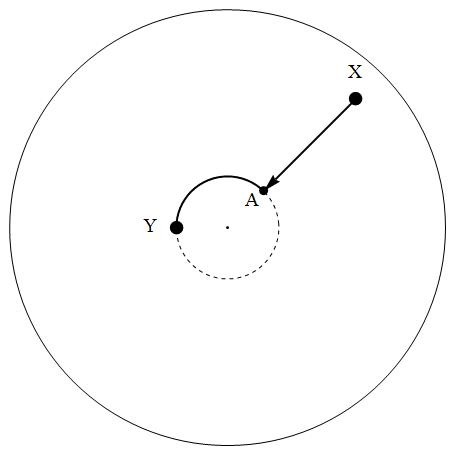
\includegraphics[width=0.25\textwidth]{figures/ShortArcStrategy.jpg}
\end{center}

Bardziej elastyczny sposób polega na otoczeniu grafiki konstrukcją \texttt{picture} (patrz Rys. \cref{fig:Lines}).
Poniżej znajduje się \cref{fig:Lines}. \par
Szablon pracy dyplomowej wykorzystuje pakiet \texttt{cleveref}. Służy on do elastycznego operowania referencjami wewnątrz dokumentu.  Na przykład, używając komendy \texttt{cref} (zamiast standardowej \verb|\ref{fig:Lines}|), 
nie musisz samemu pisać skrótu \texttt{Rys.}

\begin{figure}[ht]
  \centering
  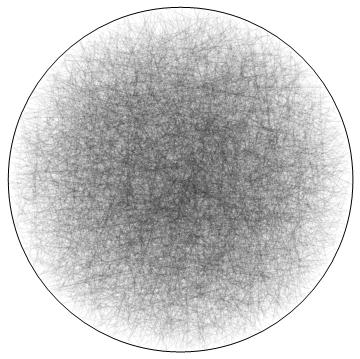
\includegraphics[scale=0.45]{figures/RandomLines.jpg}
  \caption{Symulacje 10000 losowych odcinków w kółku jednostkowym. Rysunek został samodzielnie wygenerowany.}
	\label{fig:Lines}
\end{figure}

Jeśli odkomentujesz polecenie \verb|\listoffigures| w głównym pliku, 
to rysunek ten znajdzie się na wygenerowanej liście rysunków.

\section{Wzory matematyczne}

Wzory matematyczne w obrębie paragrafu formatuje się za pomocą polecenia 
\verb|$ ... $|, np. $f(x) = \sin(x^2)$.
Za pomocą polecenia \verb|\[ ... \]| formatujesz równania wycentrowane bez numerowania, np.
\[
  \sin^2(\alpha) + \cos^2(\alpha) = 1 ~,
\]
a za pomocą konstrukcji \verb|\begin{equation} ... \end{equation}| 
formatujesz równania numerowane, np.
\begin{equation} \label{eq:ExpFnc}
 \exp(I \cdot t) = \cos(t) + I\cdot\sin(t)
\end{equation}
Równań numerowanych używaj \textbf{tylko wtedy}, gdy będziesz się do nich odwoływać w dalszej części tekstu 
za pomocą polecenia \verb|\ref{...}|.  

Jeśli w pracy znajdą się jakieś twierdzenia, lematy, to skorzystaj z konstrukcji \texttt{theorem}, \texttt{lemma}, \texttt{corollary}   oraz \texttt{proof}, zdefiniowanych w pakiecie \texttt{amsthm}, zaimportowanym do tego szablonu. Oto przykład:

\begin{theorem}[Euklides]
Istnieje nieskończenie wiele liczb pierwszych.
\end{theorem}

\begin{proof} 
Załóżmy, że $p_1,\ldots,p_n$ jest listą wszystkich liczb pierwszych. Niech
\[
  q = (p_1\cdot\cdots\cdot p_n) + 1 ~.
\]
Wtedy $q>1$, istnieć więc musi liczba pierwsza $p$ taka, że $p|q$. ...
\end{proof}

\section{Cytowania}
\label{examples:cite}

W tym szablonie korzystamy z biblioteki \texttt{biber} do formatowania cytatów. 
Jest to nowocześniejsza wersja standardowej (ale obecnie już nie rozwijanej) biblioteki \texttt{bibtex}.
Oto przykład użycia:

\begin{quote}
   Książka \cite{KNUTH01} jest poświęcona podstawowym algorytmom. 
   Autor \citeauthor{KNUTH01} omawia w niej większość klasycznych algorytmów. 
   Z punktu widzenia tej pracy ważny jest algorytm znajdujący się w \textcite[249]{KNUTH02}.\par
   Prace \cite{KuhnWZ08}, \cite{PapaGeo07} zawierają zwięzłe wprowadzenia do problematyki \textit{routingu geograficznego}.
\end{quote}

Wpisy opisujące źródła bibliograficzne najlepiej jest przechowywać w oddzielnym pliku o formacie \texttt{bibtex}. 
Do szablonu dołączony jest przykładowy plik \texttt{bibliography.bib}. Znajdują się w nim przykłady podstawowych typów tzw. wpisów.
Porządnie sformatowane wpisy bibliograficzne możesz znaleźć, na przykład, na stronach 
\href{https://dblp.org/}{dblp} oraz w serwisie \href{https://scholar.google.com/}{Google Scholar}. \par


Biber, używany z pakietem biblatex, zapewnia wiele predefiniowanych stylów formatowania cytatów i bibliografii, z typowymi stylami takimi jak  
\texttt{numeric}, \texttt{alphabetic}, \texttt{authoryear}, \texttt{authortitle} i \texttt{verbatim}, 
wraz z opcjami sortowania, takimi jak \texttt{nty} (name, title, year) lub \texttt{nyt} (name, year, title). 
Style te są wybierane za pomocą opcji \texttt{style=} w poleceniu 
\begin{center}
\verb|\usepackage[backend=biber, style=...]{biblatex}| 
\end{center}
w preambule Latex'a. Stosowany w pracy styl formatowania ustal wspólnie z opiekunem pracy. W pliku \texttt{main.tex} zaproponowano styl numeryczny bez opcji sortowania, co oznacza, że bibliografia będzie wyświetlana w kolejności pojawienia się cytowanej pozycji w tekście pracy. 

\subsection*{Uwaga} Cytowania w Latex'u możesz samodzielnie obsługiwać bez pomocy pliku w formacie bibtex. Jednak samodzielne, poprawne sformatowanie bibliografii jest dość żmudne. Pamiętaj również o tym, że każda pozycja występująca w spisie literatury musi być cytowana w tekście pracy.  

\section{Tabele}

Tabele wstawiasz w sposób standardowy. 
Po odkomentowaniu polecenia  \verb|\listoftables| z głównego pliku tego szablonu do pliku zostanie dołączona lista tabel.
Do tej tabeli możesz się odwoływać za pomocą polecenia \verb|\cref{tab:example}| (\cref{tab:example}).
                                             
\begin{table}[htbp]
  \caption{Przykładowa tabela }
  \centering
  \begin{tabular}{|l|l|r|}
    \hline
    \textbf{Kategoria} & \textbf{Parametr} & \textbf{Wynik} \\
    \hline
    Test A & Niskie obciążenie & 15 ms \\
    Test B & Wysokie obciążenie & 120 ms \\
    \hline
  \end{tabular}
  \label{tab:example}
\end{table}

\section{Kody procedur}

Do tego szablonu dołączony został pakiet \texttt{listings}. 
Ułatwia on wstawianie kodów źródłowych do dokumentu. W szablonie, w pliku \texttt{ustawienia.tex},  
są ustawione domyślne parametry wyświetlania dla kodów. 

Oto przykład jego użycia:

\begin{lstlisting}[language=C, 
caption={Algorytm Euklidesa w języku C}, 
label={lst:hello}]
/* 
 * Algorytm Euklidesa.
 * Zwraca gcd(a, b).
 */
int gcd(int a, int b)
{
    while (b != 0) {
        int r = a % b;
        a = b;
        b = r;
    }
    return a;
}
\end{lstlisting}

Oto inny przykład, kod implementacji algorytmu QuickSort w języku Haskell (\cref{lst:hhaskell:qs}) wykorzystujący,
dla zwiększenia czytelności kodu,  mechanizm \textit{list comprehension}: \par

\begin{lstlisting}[style=haskellStyle, %language=haskell, 
caption={Algorytm QuickSort w języku Haskell}, 
label={lst:hhaskell:qs}]
-- QuickSort: czas O(n^2); średni czas O(n log(n))
qs [] = []
qs (x:xs) = qs [t| t<- xs, t < x] ++ 
            [x] ++ 
						qs [t| t<- xs, t >= x]
\end{lstlisting}


Do wstawiania pseudokodów do pracy zalecamy korzystanie z pakietów \texttt{algorithm} oraz \texttt{algpseudocode} dołączonych do tego szablonu.
Oto przykład pseudokodu zapisanego w języku tych pakietów (\cref{ps:filtr}):


\begin{algorithm}[H]
\caption{Filtrowanie}
\label{ps:filtr}
\begin{algorithmic}[1]
\State Initialize: $S \gets \emptyset$
\For{$v \in V$}
  \If{$\mathrm{condition}(v)$}
    \State $S \gets S \cup \{v\}$ \Comment{Dodaj jeśli spełnia warunek}
  \EndIf
\EndFor
\State \Return $S$
\end{algorithmic}
\end{algorithm}

\section{Akronimy}

Szablon ten korzysta z pakietu \texttt{acro}. Plik \texttt{acronims.tex} jest przykładem pliku konfiguracyjnego.
Oto przykład użycia:
\begin{quote}
  Podczas budowania oprogramowania dużą wagę przykładaliśmy do przestrzegania dwóch 
	zasad: zasady \ac{dry} oraz zasady \ac{kiss} 
\end{quote}
Za drugim razem, gdy użyjesz synonimów, pojawią się już tylko skrócone nazwy, na przykład:
\begin{quote}
  Stosowanie zasady \ac{dry} polega unikaniu pisania kilkukrotnie podobnych fragmentów kodu.  Stosowanie tej zasady znacznie ułatwia modyfikację kodów. 
  Z kolei stosowanie zasady \ac{kiss} zmusza programistę do systematycznego zastanawiania się nad jakością swojego kodu.
\end{quote}

Jeśli nie masz potrzeby korzystania z akronimów, to zakomentuj dwie linie w pliku \texttt{main.tex} (linie 59 oraz 73).
 
